\subsection{استخراج قسمت های کوچیک تر از یک اسلاید}\label{subsec:استخراج-قسمت-های-کوچیک-تر-از-یک-اسلاید}

اسلاید هایی که متخصصان از آن برای تشخیص استفاده می کنند بسیار ابعاد بزرگی دارند، به طوری که به هیچ وجه در
حافظه پردازنده ها جای نمی گیرد.
برای حل این مشکل در این پروژه سعی بر این شد که اسلاید ها به تیکه های کوچک تری از عکس شکسته شوند به طوری که قابل پردازش باشند.
یکی از موضوعات مهمی که باید در نظر گرفت، ناحیه های غیر مهم و فاقد اطلاعات است که باید در این فرآیند حذف گردند. این کار به دو دلیل انجام می شود.
اولا اینکه این قسمت ها، بخش بزرگی از اسلاید ها را تشکیل می دهند و با حذف این موارد می توان در استفاده از منابع پردازشی صرفه جویی کرد
و دوما اگر تعداد زیادی از عکس هایی که هنگام آموزش مدل استفاده می کنیم، از این نوع باشند، دقت مدل بشدت کاهش پیدا می کند و مدل در فرآیند یادگیری با مشکل مواجه می شود.
دلیل این امر هم این است که این عکس ها حاوی ویژگی های مورد نظر ما برای تشخیص سلول های سرطانی نیستند و مدل در حین فرآیند آموزش، ویژگی های نامربوطی را از روی این عکس ها یاد می گیرد.

برای حل این موضوع، روشی که بکار گرفته شد، استفاده از واریانیس لاپلاسین ناحیه است.
لاپلاسین یک عکس از محاسبه مشتق دوم روی شدت رنگ های پیکسل های آن محاسبه می شود
و در نتیجه لبه و گوشه های عکس مقدار بیشتری می گیرد.
برای محاسبه مشتق دوم برای یک عکس از رابطه زیر استفاده می کنیم که در آن $f(x)$ مقدار شدت رنگ را در موقعیت x از تصویر نشان می دهد.

\begin{gather*}
    f'(x) = f(x+1) - f(x), f'(x+1) = f(x+2) - f(x+1)\\
    f"(x) = f'(x+1) - f'(x)= f(x+2) - f(x+1) - f(x+1) + f(x)\\
    f"(x) = f(x+2) - 2*f(x+1) + f(x)\\
\end{gather*}

بعد از محاسبه واریانس شدت رنگ پیکسل ها در لاپلاسین عکس و استفاده از یک آستانه عکس هایی که مقدار کمتری دارند فیلتر می شوند.
به این ترتیب ناحیه های فاقد اطلاعات که مقدار لاپلاسین کمی نیز دارند حذف می شوند.

برای بدست آوردن مقدار بهینه آستانه و همچنین آزمودن این روش، برای شش تا از اسلاید ها به صورت دستی، ماسک هایی از ناحیه های دارای اطلاعات تهیه شد.
همانطور که در قسمت قبل گفته شد، فیلتر ناحیه های فاقد اطلاعات، اهمیت زیادی برای ما دارد از این رو در ارزیابی این روش علاوه بر دقت، تمایزگری\LTRfootnote{Specificity}، عامل مهمی در کارکرد درست است.
این معیار با توجه به فرمول زیر هرچه به مقدار عددی 1 نزدیک تر باشد بهتر است و به این معناست که ناحیه های بدست آمده از این روش، به احتمال بالاتری دارای اطلاعات هستند و در نتیجه ناحیه های فاقد اطلاعات کمتری تولید می شوند.
\begin{gather*}
    TruePositive =\textit{روش به درستی عکس را غیر پس زمینه تشخیص داده}\\
    TrueNegative =\textit{ روش به درستی عکس را پس زمینه تشخیص داده}\\
    FalsePositive =\textit{ روش اشتباهاً عکس را غیر پس زمینه تشخیص داده}\\
    FalseNegative =\textit{ روش اشتباهاً عکس را پس زمینه تشخیص داده}\\
    Specificity = \frac{TruePositive}{TruePositive + FalsePositive}\\
\end{gather*}
دقت روش نیز به صورت زیر محاسبه می شود:
\[Accuracy = \frac{TP + TN}{TP + FP + TN + FN}\]
برای این کار قطعه کد پایتونی نوشته شد که 6 اسلاید و ماسک های مربوط به آن ها را به عنون ورودی می گیرد و با مقدار دهی اولیه آستانه به اندازه 250 و محاسبه ماتریس درهم ریختگی\LTRfootnote{Confusion Matrix} در جهتی آستانه را تغییر می دهد تا دو معیار گفته شده بیشینه شوند.
اسلاید ها و ماسک های بکار رفته آن ها در تصویر~\رجوع{شکل: سه اسلاید و ماسک های مرتبط} ارائه شده است.
در نهایت برای مشاهده دقت و حساسیت روش بر روی این سه اسلاید می توانید به جدول~\رجوع{جدول: دقت روش لاپلاسین بر روی سه اسلاید} رجوع کنید.
\begin{table}[t]
    \centering
    \begin{latin}
        \begin{tabular}{|c|c|c|c|c|}
            \hline
            \rl{اسلاید} & \rl{دقت} & \rl{حساسیت} & \rl{تعداد کل عکس ها} & \rl{تعداد عکس های خروجی}
            \\
            \hline
            \hline
            \textit{a} & $0.69$ & $0.90$ & 1500 & 666\\
            \textit{b} & $0.97$ & $0.95$ & 5110 & 2917\\
            \textit{c} & $0.82$ & $0.99$ & 1750 & 1119\\
            \hline
        \end{tabular}
    \end{latin}
    \caption{دقت روش لاپلاسین برای تشخیص عکس های پس زمینه از غیر پس زمینه و تعداد عکس های هر اسلاید}
    \label{جدول: دقت روش لاپلاسین بر روی سه اسلاید}
\end{table}

\begin{figure}
    \begin{center}

        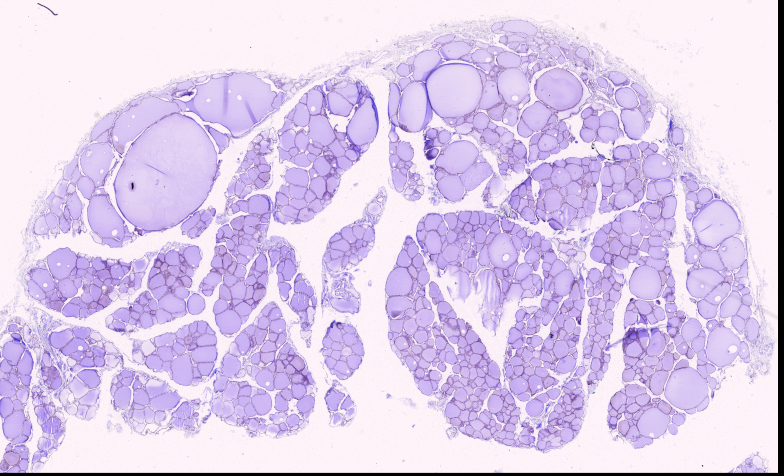
\includegraphics[width=0.48\linewidth]{figs/687_resized.jpg}
        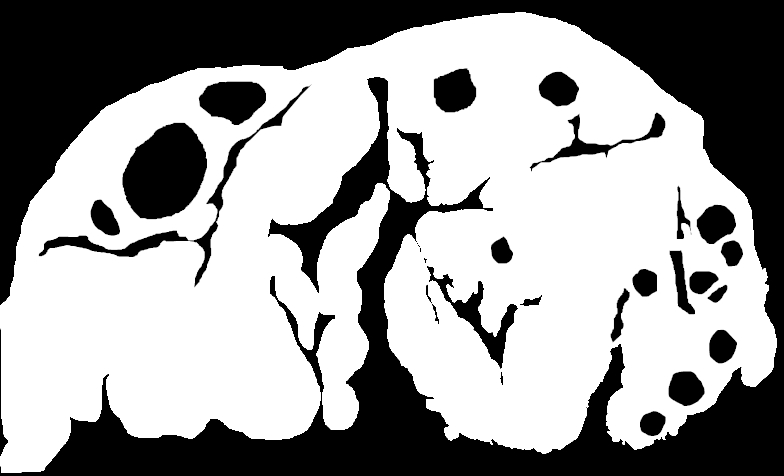
\includegraphics[width=0.48\linewidth]{figs/687_mask_resized.jpg}
        \hspace{.5cm}

        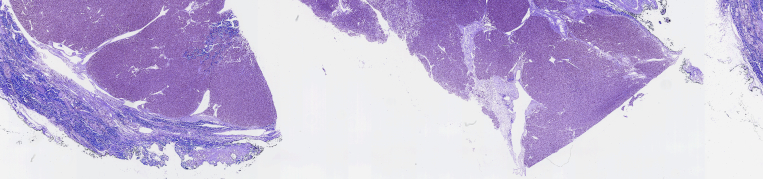
\includegraphics[width=0.48\linewidth]{figs/1066_cropped_resized.jpg}
        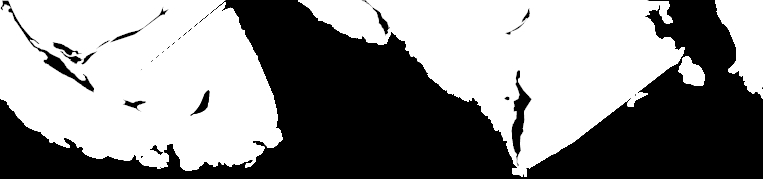
\includegraphics[width=0.48\linewidth]{figs/1066_cropped_masked_resized.jpg}
        \hspace{.5cm}

        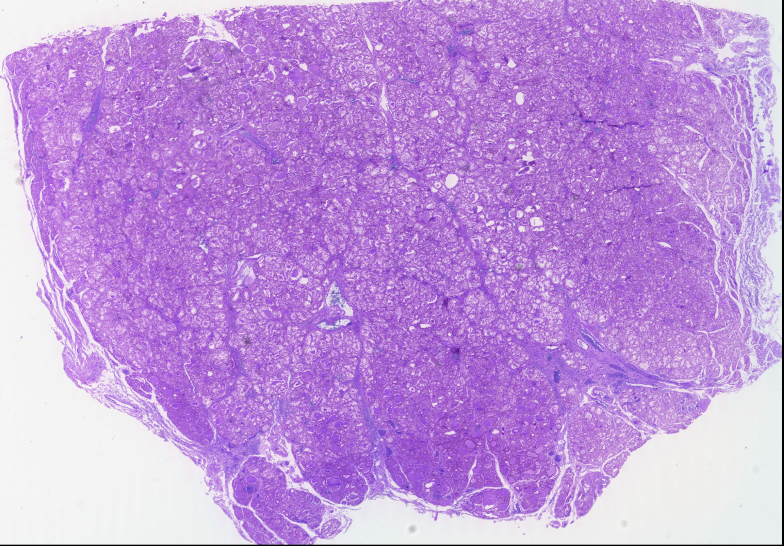
\includegraphics[width=0.48\linewidth]{figs/575_resized.jpg}
        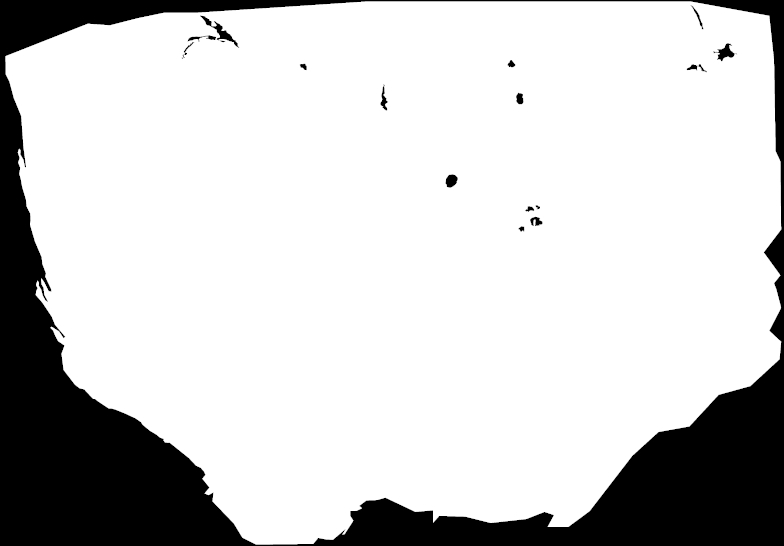
\includegraphics[width=0.48\linewidth]{figs/575_mask_resized.jpg}


    \end{center}
    \caption{سه اسلاید $a$, $b$, $c$ و ماسک های مرتبط}
    \label{شکل: سه اسلاید و ماسک های مرتبط}
\end{figure}

یکی از مزیت های این روش نسبت به روش دیگر این است که ناحیه های تار شده و خارج از فکوس را نیز فیلتر می کند.
این اتفاق به دلایل مختلفی ممکن است پیش بیاید.
ممکن است دستگاه اسکنر مشکلی داشته باشد یا ممکن است لام به درستی قرار نگرفته باشد.
به هر حال، در صورتی که ناحیه ای از اسلاید تار شده باشد و ناحیه اطلاعات خود را از دست داده باشد،
توسط این روش فیلتر می شود زیرا ناحیه های تار معمولا واریانس کمتری در شدت رنگ خود دارند.

